\documentclass{article}
\usepackage{graphicx}
\usepackage[top=0.75in, bottom=0.75in, left=0.75in, right=0.75in]{geometry}

\begin{document}

\title{Text Technologies for Data Science: Assessment 4}
\author{s1107496}

\maketitle

\section{Introduction}
This report describes the analysis of the Enron email dataset via implementation of the PageRank and Hubs \& Authorities algorithms. It also describes the further automatic identification and visualization of key players and topics at Enron.

\section{PageRank and Hubs \& Authorities}
For both PageRank and Hubs \& Authorities, the data were initially converted into a graph, with email addresses as nodes linked by weighted, directional edges representing emails sent.
\subsection{PageRank}
The standard PageRank algorithm was implemented, with $\lambda$ set to 0.8. A slight modification to the algorithm was made to account for edge weighting. Sink nodes were identified before running the algorithm, and these were accounted for as per the lecture slides given in Text Technologies for Data Science. The PageRank algorithm was run for 10 iterations.
\subsection{Hubs \& Authorities}
The standard algorithm for Hubs \& Authorities as presented in Text Technologies for Data Science was implemented, with a slight modification made to account for edge weighting. The Hubs \& Authorities algorithm was run for 20 iterations.

\section{Key players}
\subsection{Identification}
To identify key players at Enron, the following steps were taken. First, the message identifiers as supplied in graph.txt were linked to their respective subjects as provided in subject.txt. For each token appearing in the text of the subjects, an IDF value was calculated. Following this, the 50 most common tokens as measured by IDF were combined with the English-language stopwords provided by the \texttt{nltk} library to create a domain-specific set of stopwords.

Having calculated the PageRanks for all email addresses (as described in the preceding section), the top 10 emails by PageRank were selected. These were considered likely candidates to be "important" Enron figures. On the assumptions that A) the most "important" figures at Enron may not synonymous with key figures in an investigative sense and B) "important" figures are most likely to email each other about important topics, the top 50 most commonly used terms in emails between important figures were used as a query. Further to this, for each email address, a document was created consisting of all subjects sent to and from that email address. 

Finally, a PageRank-weighted version of TF-IDF was implemented and used to find figures that best matched the query while still having high PageRank scores. The top 10 results from this retrieval task are compared to the top 10 results by PageRank below.
\begin{figure}
\begin{tabular}{l | l | l}
Rank & PageRank & PageRank-weighted TF-IDF \\
\hline
1 & klay@enron.com & tana.jones@enron.com \\
2 & jeff.skilling@enron.com & sara.shackleton@enron.com \\
3 & sara.shackleton@enron.com & mark.taylor@enron.com \\
4 & tana.jones@enron.com & louise.kitchen@enron.com \\
5 & mark.taylor@enron.com & gerald.nemec@enron.com \\
6 & kenneth.lay@enron.com & jeff.skilling@enron.com \\
7 & louise.kitchen@enron.com & kenneth.lay@enron.com \\
8 & gerald.nemec@enron.com & john.lavorato@enron.com \\
9 & jeff.dasovich@enron.com & elizabeth.sager@enron.com \\
10 & sally.beck@enron.com & marie.heard@enron.com \\

\end{tabular}
\end{figure}

As can be seen, jeff.dasovich@enron.com, sally.beck@enron.com, and klay@enron.com (an alternate email for Kenneth Lay) were not present in the top 10 figures by TF-IDF, having been replaced by elizabeth.sager@enron.com, john.lavorato@enron.com, and marie.heard@enron.com.

\subsection{Visualization}
To visualize the communications between key figures, a weighted directional graph was created using the Python library \texttt{networkx}. Nodes are separated in space such that nodes with more frequent communication are located more closely together. For each connected pair of nodes, the top 3 non-numeric non-stopwords used in their communications were used to label the edge. 

\begin{figure}[ht!]
\centering
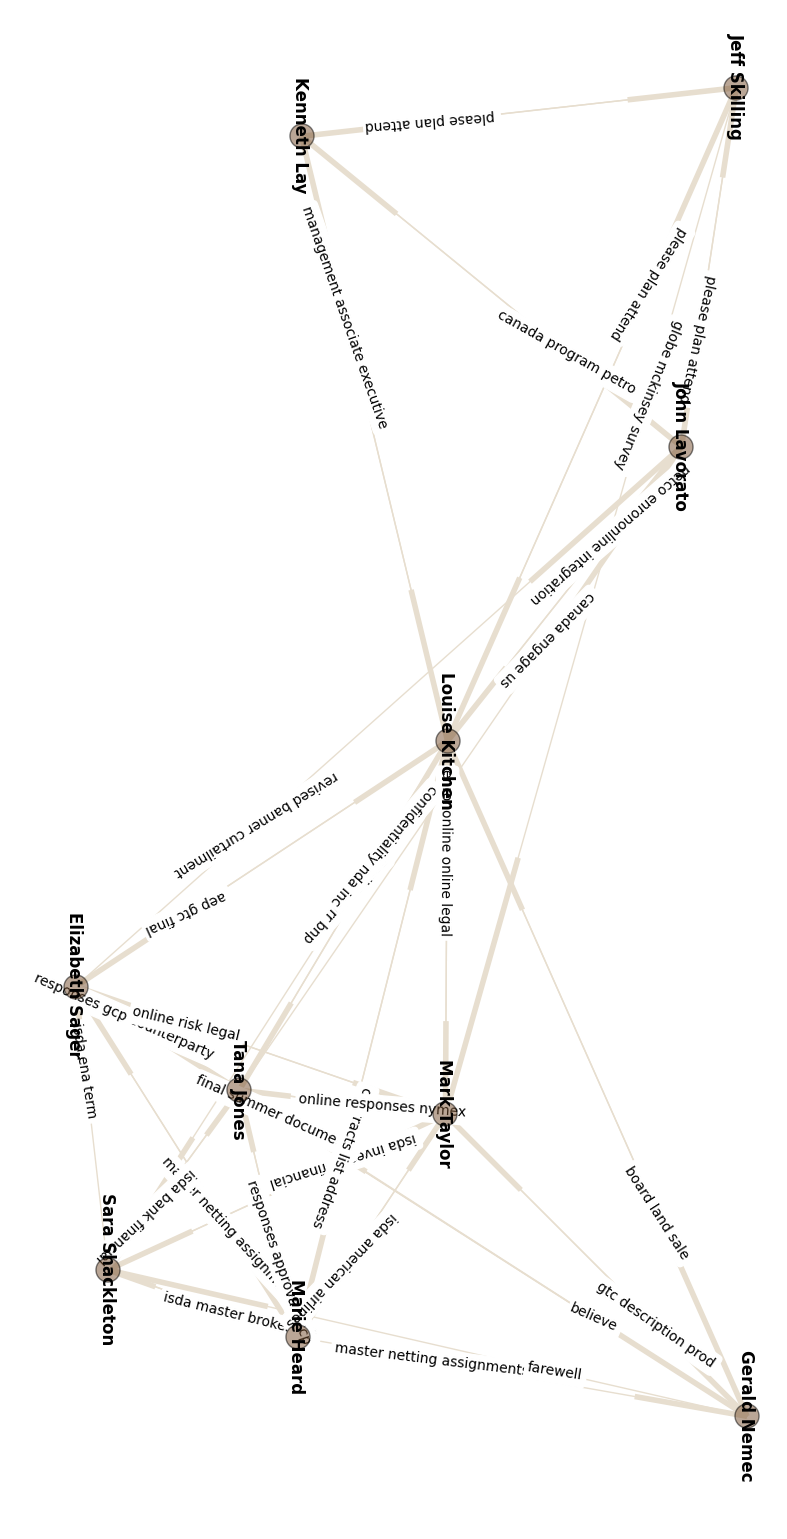
\includegraphics[height=260mm]{graph.png}
\end{figure}

\end{document}